\documentclass[11pt]{article}
\usepackage[a4paper,margin=26mm]{geometry}
\usepackage[T1]{fontenc}
\usepackage{lmodern}
\usepackage{amsmath,amssymb,amsthm}
\usepackage{microtype}
\usepackage{array}
\usepackage{tikz}
\usetikzlibrary{calc}
\usepackage{xurl}
\usepackage{hyperref}
\hypersetup{colorlinks=true,linkcolor=blue,urlcolor=blue,citecolor=blue,
 pdftitle={Arbitrarily large antichains of trees of equal order in the independence polynomial order},
 pdfauthor={Horace Dong}}
\newtheorem{theorem}{Theorem}
\newtheorem{lemma}{Lemma}
\newtheorem{proposition}{Proposition}
\newtheorem{corollary}{Corollary}
\theoremstyle{definition}
\newtheorem{definition}{Definition}
\theoremstyle{remark}
\newtheorem{remark}{Remark}
\newcommand{\repoversion}{1.25.0}
\setlength{\emergencystretch}{1.5em}
\newcommand{\sA}{\mathsf A}
\newcommand{\sB}{\mathsf B}
\newcommand{\sO}{\mathsf O}

\title{Arbitrarily large antichains of trees of equal order\\ in the independence polynomial order}
\author{Horace Dong\\ \small Independent researcher\\
\small\texttt{maxwelldhx@gmail.com}\\
\small ORCID: \href{https://orcid.org/0009-0002-7554-7548}{0009-0002-7554-7548}}
\date{22 November 2026}
\begin{document}
\maketitle

\begin{abstract}
The independence polynomial $I(G,x)$ of a graph $G$ counts the independent
sets of $G$ by size, and $\xi(G)$ denotes its largest real root. Csikvári
introduced the relation $H\preceq G$, which in the form used by Beaton and
Cameron holds when $I(H,x)\ge I(G,x)$ for
all $x\in[\xi(G),0]$. Beaton and Cameron showed that two trees of the same
order need not be comparable, by giving pairs of incomparable trees, and asked
whether there can be arbitrarily large antichains with respect to $\preceq$
among trees of equal order. We answer this question in the affirmative: for
every $n\ge 11$ there are $\lfloor n/11\rfloor+1$ trees on $n$ vertices that
are pairwise incomparable. The trees are paths in which every vertex except
at most ten carries one of two ten-vertex gadgets, $A$ or $B$. Replacing one
gadget $B$ by a gadget $A$ lowers the independence polynomial at
$-1/10$ and raises it at $-1/6$, and both points lie in the comparison interval
of every tree of the family. The result
is formally verified in Lean~4. The proofs were found and formalized by AI
agents working under the author's direction; their role is described at the
end of the paper.
\end{abstract}

\section{Introduction}

All graphs are finite, simple and undirected. A set of vertices of a graph $G$
is \emph{independent} if no two of its vertices are adjacent. The
\emph{independence polynomial} of $G$ is
\[
I(G,x)=\sum_{k\ge0} i_k(G)\,x^k ,
\]
where $i_k(G)$ is the number of independent sets of size $k$ in $G$; the empty
set is counted, so $I(G,0)=1$. The roots of $I(G,x)$ are the
\emph{independence roots} of $G$. Beaton and Cameron~\cite{bc} write $\xi(G)$
for the independence root of smallest modulus; citing a note of Csikvári~\cite{cs2}, they note that
for every graph it is real and lies in $[-1,0)$, and therefore coincides with
the largest real independence root~\cite[p.~30]{bc}. We work throughout with
the largest real root, which we also denote by $\xi(G)$; for the trees used
below its existence is proved directly (Lemma~\ref{lem:root}).

Following Csikvári~\cite[Section~8]{cs}, who works with $I(G,-x)$ and its
smallest positive root, in the form used by Beaton and
Cameron~\cite[p.~31]{bc}, define
\[
H\preceq G \quad\Longleftrightarrow\quad I(H,x)\ge I(G,x)\ \text{ for all }
x\in[\xi(G),0].
\]
Note that the interval is determined by the graph on the right. Two graphs $G$
and $H$ are \emph{comparable} if $H\preceq G$ or $G\preceq H$, and
\emph{incomparable} otherwise. Graphs with the same independence polynomial
are called independence equivalent, and the relation $\preceq$ induces a
partial order on the set of independence equivalence classes~\cite[Theorem~1]{bc},
transitivity being due to Csikvári~\cite[Section~8]{cs}. Csikvári also showed that, among the trees of
a given order $n$, the path is the unique minimum and the star the unique
maximum with respect to~$\preceq$ (as reported in~\cite[Section~4]{bc}). The
same relation appears in Oboudi's preprint~\cite{ob}, which proves a corresponding
extremal result for trees and conjectures that any two trees of the same order
are comparable~\cite[Conjecture~1]{ob}. Beaton and Cameron, citing the journal paper~\cite{ob18}, disproved this
conjecture~\cite[Section~3.1]{bc}: they found two incomparable trees of order~$8$ and, applying the
graph star operation to both, two incomparable trees of order $2^{k+3}$ for
every $k\ge0$ \cite[Figure~16 and Theorem~16]{bc}. They then asked:

\begin{quote}
\textbf{Question 6 of~\cite{bc}.} Can there be arbitrarily large anti-chains
with respect to $\preceq$ among trees of equal order?
\end{quote}

\noindent Throughout we use the numbering of the journal version~\cite{bc}.
In the arXiv version (arXiv:2006.05511v2) the same items are Question~5.3,
Theorem~4.6 and Figure~17, and the partial-order result is Theorem~1.1.
We answer the question in the affirmative.

\begin{theorem}\label{thm:main}
For every integer $n\ge 11$ there exist $\lfloor n/11\rfloor+1$ trees on $n$
vertices that are pairwise incomparable with respect to $\preceq$. Their
independence polynomials are pairwise different; in particular the trees are
pairwise non-isomorphic, and their independence equivalence classes form an
antichain of size $\lfloor n/11\rfloor+1$ in the partial order of these
classes.
\end{theorem}

\begin{corollary}\label{cor:arb}
For every $k\ge1$ there is an order $n$ (for instance $n=11k$) such that some
$k$ trees on $n$ vertices are pairwise incomparable with respect to $\preceq$.
\end{corollary}

\noindent The trees of Theorem~\ref{thm:main} can be chosen with maximum
degree at most~$5$ (Remark~\ref{rem:degree}); this property is proved only in
the text and is not part of the Lean statements.

The construction is explicit. Two rooted trees $A$ and $B$ on ten vertices are
obtained from the same nine-vertex tree by attaching a leaf at two different
vertices. A path is decorated by attaching a copy of $A$ or of $B$ at each of
$m$ of its vertices (and nothing at up to ten further vertices), and the
$m+1$ trees in which the leftmost $j$ gadgets are $A$ and the others $B$
($0\le j\le m$) form the antichain. Exchanging one $B$ for an $A$ changes the
independence polynomial by $x^3\bigl((2+x)(1+x)^4-1\bigr)$ times a product of
two independence polynomials (Lemma~\ref{lem:swap}). This factor is negative
at $x=-1/10$ and positive at $x=-1/6$. The other step is to show that both test
points lie in the comparison interval of every tree in the family, which
amounts to showing that no independence polynomial in the family vanishes on
$[-1/6,0]$ (Lemma~\ref{lem:pos}); this is done with a two-term transfer
recursion along the path and three polynomial inequalities with explicit
certificates.

\subsection*{Prior work}
The relation $\preceq$ and the extremal trees are due to Csikvári~\cite{cs};
see also~\cite{ob}. Beaton and Cameron's pair of order~$8$~\cite[Figure~16]{bc} is
certified in the same way as here, by two points in the common comparison
interval at which the values of the two independence polynomials are in
opposite order (they use $-0.1$ and $-0.2$); the pairs of larger order
in~\cite[Theorem~16]{bc} are obtained from it with the graph star
operation~\cite[Lemma~2]{bc}. Their pairs give antichains of size two at infinitely many orders;
the construction above gives antichains whose size grows linearly with the
order, at every order $n\ge11$. As far as we know, Question~6 of~\cite{bc}
has not been answered elsewhere; the searches are described in the final
section.

\section{The construction}\label{sec:construction}

\paragraph{The gadgets.}
Let $H$ be the tree on nine vertices obtained from a path $u - v - s$ by
attaching two leaves to $u$ and four leaves to $s$. Let $A$ be the tree
obtained from $H$ by adding a new vertex $r$ adjacent to $u$, and let $B$ be
obtained from $H$ by adding a new vertex $r$ adjacent to $v$. We regard $A$
and $B$ as rooted at $r$; both have ten vertices, and $A-r=B-r=H$. (This
tree $H$ is unrelated to the generic graph $H$ in the definition
of~$\preceq$.)

\paragraph{Decorated paths.}
A \emph{word} is a finite sequence $w=w_1w_2\cdots w_k$ of letters from the
alphabet $\{\sA,\sB,\sO\}$. For a nonempty word $w$, the tree $T(w)$ consists
of a path $p_1p_2\cdots p_k$ (the \emph{spine}) together with, for every $i$
with $w_i=\sA$ (resp.\ $w_i=\sB$), a disjoint copy of $A$ (resp.\ $B$) whose
root $r$ is joined to $p_i$ by an edge; positions with $w_i=\sO$ carry nothing.
Each step adds a tree joined by one edge to the tree built so far, so $T(w)$
is a tree. It has $11a+c$ vertices, where $a$ is the number of letters
$\sA$ or $\sB$ in $w$ and $c$ the number of letters~$\sO$. Figure~\ref{fig:sites}
shows the two kinds of decorated spine vertices.

\begin{figure}[ht]
\centering
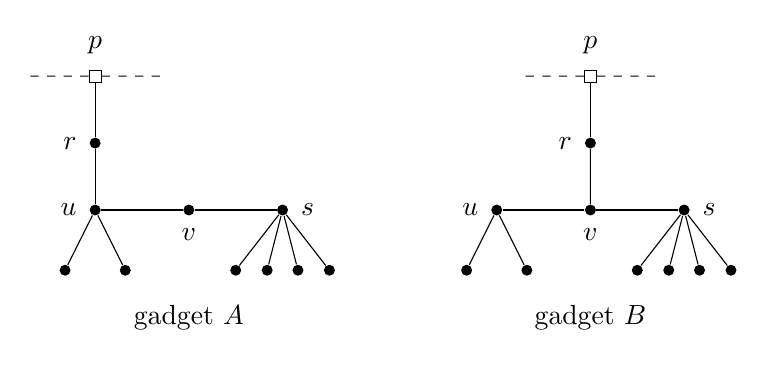
\begin{tikzpicture}[v/.style={circle,fill,inner sep=1.4pt},
  w/.style={rectangle,draw,fill=white,inner sep=2.2pt},scale=0.85]
\foreach \dx/\att/\name in {0/u/A,6/v/B}{
\begin{scope}[xshift=\dx cm]
 \node[v,label={[label distance=1pt]left:$u$}] (u) at (0,0) {};
 \node[v,label={[label distance=1pt]below:$v$}] (v) at (1.4,0) {};
 \node[v,label={[label distance=1pt]right:$s$}] (s) at (2.8,0) {};
 \draw (u)--(v)--(s);
 \foreach \x in {-0.45,0.45} {\node[v] (l) at (\x,-0.9) {}; \draw (u)--(l);}
 \foreach \x in {2.1,2.57,3.03,3.5} {\node[v] (l) at (\x,-0.9) {}; \draw (s)--(l);}
 \node[v,label={[label distance=1pt]left:$r$}] (r) at ($(\att)+(0,1)$) {};
 \draw (\att)--(r);
 \node[w,label={[label distance=2pt]above:$p$}] (p) at ($(\att)+(0,2)$) {};
 \draw (r)--(p);
 \draw[dashed] (p)--++(-1,0); \draw[dashed] (p)--++(1,0);
 \node at (1.4,-1.6) {gadget $\name$};
\end{scope}}
\end{tikzpicture}
\caption{The two decorated spine vertices. The tree $H$ consists of $u$, $v$,
$s$ and six leaves. Gadget $A$ (left) has its root $r$ joined to $u$, gadget
$B$ (right) has $r$ joined to $v$. The spine vertex $p$ (square) is joined to
$r$; dashed edges lead to the neighbouring spine vertices.}
\label{fig:sites}
\end{figure}

\paragraph{The family.}
Let $n\ge11$, $m=\lfloor n/11\rfloor\ge1$ and $\ell=n-11m\in\{0,1,\dots,10\}$.
For $0\le j\le m$ let
\[
T_j=T\bigl(\sA^{j}\,\sB^{m-j}\,\sO^{\ell}\bigr),
\]
the decorated path whose leftmost $j$ spine vertices carry $A$, the next $m-j$
carry $B$ and the last $\ell$ carry nothing. Each $T_j$ is a tree on
$11m+\ell=n$ vertices. Theorem~\ref{thm:main} asserts that
$T_0,T_1,\dots,T_m$ are pairwise incomparable.

\begin{remark}\label{rem:degree}
In $T_j$ the vertex $s$ of each gadget has degree~$5$, the vertex $u$ has degree
at most $4$, $v$ at most $3$, the root $r$ degree~$2$, every spine vertex at
most $3$, and all other vertices are leaves. So the maximum degree of $T_j$ is
$5$. This remark is not stated in the Lean files.
\end{remark}

\section{Independence polynomials of decorated paths}\label{sec:poly}

We write $I(G)$ for $I(G,x)$ when the variable is clear; the independence
polynomial of the graph with no vertices is~$1$. We use the standard vertex
recurrence: for every vertex $y$ of $G$,
\begin{equation}\label{eq:vertex}
I(G)=I(G-y)+x\,I(G-N[y]),
\end{equation}
where $N[y]$ is the closed neighbourhood of $y$; the two terms count the
independent sets not containing $y$ and containing $y$. Moreover the
independence polynomial of a disjoint union is the product of those of the
components.

\begin{lemma}\label{lem:gadget}
The gadgets have the independence polynomials
\begin{align*}
I(H)&=1+9x+28x^2+42x^3+39x^4+22x^5+7x^6+x^7,\\
I(A)&=1+10x+36x^2+65x^3+75x^4+57x^5+28x^6+8x^7+x^8,\\
I(B)&=1+10x+36x^2+64x^3+66x^4+41x^5+14x^6+2x^7,
\end{align*}
and
\begin{equation}\label{eq:diff}
I(A)-I(B)=x^3\bigl((2+x)(1+x)^4-1\bigr).
\end{equation}
In particular
\[
I(A)-I(B)=-\tfrac{24659}{100000000}<0 \ \text{ at } x=-\tfrac1{10},
\qquad
I(A)-I(B)=\tfrac{901}{1679616}>0 \ \text{ at } x=-\tfrac16 .
\]
\end{lemma}

\begin{proof}
The polynomials are obtained from~\eqref{eq:vertex} by direct computation. For
the difference, apply~\eqref{eq:vertex} at $r$: $I(A)=I(H)+x\,I(H-u)$ and
$I(B)=I(H)+x\,I(H-v)$. The graph $H-u$ consists of two isolated vertices and a
star with centre $s$ and five leaves ($v$ and the four leaves of $s$), so
$I(H-u)=(1+x)^2\bigl((1+x)^5+x\bigr)$. The graph $H-v$ consists of a star with
two leaves and a star with four leaves, so
$I(H-v)=\bigl((1+x)^2+x\bigr)\bigl((1+x)^4+x\bigr)$. Hence
\begin{align*}
I(A)-I(B)&=x\Bigl[(1+x)^7+x(1+x)^2-(1+x)^6-x(1+x)^4-x(1+x)^2-x^2\Bigr]\\
&=x^2\Bigl[(1+x)^4\bigl((1+x)^2-1\bigr)-x\Bigr],
\end{align*}
which equals~\eqref{eq:diff}. At $x=-1/10$ the bracket in~\eqref{eq:diff} is
$\frac{19}{10}\cdot\frac{6561}{10000}-1=\frac{24659}{100000}>0$ and
$x^3=-\frac1{1000}$; at $x=-1/6$ it is
$\frac{11}{6}\cdot\frac{625}{1296}-1=-\frac{901}{7776}<0$ and
$x^3=-\frac1{216}$.
\end{proof}

For a letter $c$ define the polynomials $P_c$ and $Q_c$ by
\[
P_\sA=I(A),\quad P_\sB=I(B),\quad P_\sO=1,\qquad
Q_\sA=Q_\sB=x\,I(H),\quad Q_\sO=x .
\]
Thus $P_c$ counts what the decoration at a spine vertex contributes when the
spine vertex is not in the independent set, and $Q_c$ what the spine vertex and
its decoration contribute when the spine vertex is in it (then the root $r$ is
excluded, leaving $H$). For a word $w$ let $Z_w=I(T(w))$ and
$U_w=I(T(w)-p_1)$, where $p_1$ is the leftmost spine vertex, and set
$Z_\varnothing=U_\varnothing=1$ for the empty word.

\begin{lemma}[transfer recursion]\label{lem:transfer}
For every letter $c$ and every word $w$,
\[
Z_{cw}=P_c\,Z_w+Q_c\,U_w,\qquad U_{cw}=P_c\,Z_w .
\]
\end{lemma}

\begin{proof}
Let $p_1$ be the spine vertex carrying $c$ in $T(cw)$, so that $p_2$ (if $w$
is nonempty) is the leftmost spine vertex of the copy of $T(w)$. Independent
sets $S$ of $T(cw)$ with $p_1\notin S$ are unions of an independent set of
the decoration at $p_1$ and one of $T(w)$; they contribute $P_cZ_w$. If
$p_1\in S$, then $S$ contains neither $r$ (if present) nor $p_2$, and $S$ is
$\{p_1\}$ together with an independent set of $H$ (if $c\ne\sO$) and one of
$T(w)-p_2$; this contributes $Q_cU_w$. The independent sets of $T(cw)-p_1$ are
exactly those not containing $p_1$. For empty $w$ the formulas read
$Z_c=P_c+Q_c$ and $U_c=P_c$, which hold by the same argument.
\end{proof}

\section{A zero-free interval and the largest real root}\label{sec:roots}

\begin{lemma}[site bounds]\label{lem:cert}
Put $y=x+\frac16$. Then
\begin{align*}
I(H)&=\tfrac{31001}{279936}+\tfrac{117763}{46656}y+\tfrac{32555}{2592}y^2
+\tfrac{27851}{1296}y^3+\tfrac{5059}{216}y^4\\
&\qquad+\tfrac{187}{12}y^5+\tfrac{35}{6}y^6+y^7,\\
I(A)+4x\,I(H)&=\tfrac{16277}{1679616}+\tfrac{34555}{34992}y+\tfrac{179477}{11664}y^2
+\tfrac{15640}{243}y^3+\tfrac{70159}{648}y^4\\
&\qquad+\tfrac{3151}{27}y^5+\tfrac{701}{9}y^6+\tfrac{88}{3}y^7+5y^8,\\
I(B)+4x\,I(H)&=\tfrac{961}{104976}+\tfrac{71317}{69984}y+\tfrac{174745}{11664}y^2
+\tfrac{128419}{1944}y^3+\tfrac{34891}{324}y^4\\
&\qquad+\tfrac{6019}{54}y^5+\tfrac{631}{9}y^6+\tfrac{74}{3}y^7+4y^8 .
\end{align*}
Consequently, for every letter $c$ and every $x\in[-\frac16,0]$,
\[
Q_c(x)\le 0\qquad\text{and}\qquad P_c(x)+4Q_c(x)>0 ;
\]
in particular $P_c(x)>0$.
\end{lemma}

\begin{proof}
The three identities are verified by expanding the right-hand sides in powers
of $x$ and comparing with Lemma~\ref{lem:gadget}. All coefficients on the
right are positive, so for $x\ge-\frac16$ (that is, $y\ge0$) the three
left-hand sides are positive. For $c\in\{\sA,\sB\}$ and $x\in[-\frac16,0]$
this gives $Q_c=x\,I(H)\le0$ and $P_c+4Q_c>0$. For $c=\sO$ we have $Q_\sO=x\le0$
and $P_\sO+4Q_\sO=1+4x\ge\frac13$. Finally $P_c>-4Q_c\ge0$.
\end{proof}

\begin{lemma}[{no roots on $[-\frac16,0]$}]\label{lem:pos}
For every word $w$ and every $x\in[-\frac16,0]$,
\[
Z_w(x)>0,\qquad U_w(x)>0,\qquad U_w(x)\le 2Z_w(x).
\]
\end{lemma}

\begin{proof}
By induction on the length of $w$; for the empty word $Z=U=1$. Let $c$ be a
letter, assume the claim for $w$, and fix $x\in[-\frac16,0]$. Write $P=P_c(x)$,
$Q=Q_c(x)$, $Z=Z_w(x)$, $U=U_w(x)$. By Lemma~\ref{lem:cert}, $Q\le0$ and
$P+4Q>0$, so $P>0$. Since $Q\le 0$ and $U\le 2Z$, we have $QU\ge 2QZ$. Hence,
by Lemma~\ref{lem:transfer},
\[
U_{cw}=PZ>0,\qquad
Z_{cw}=PZ+QU\ge (P+2Q)Z\ge (P+4Q)Z>0,
\]
and
$2Z_{cw}-U_{cw}=PZ+2QU\ge (P+4Q)Z>0$.
\end{proof}

\begin{lemma}[largest real root]\label{lem:root}
Every tree $T$ has a largest real independence root $\xi(T)$, and
$\xi(T)<0$.
\end{lemma}

\begin{proof}
For a rooted tree $(X,\rho)$ write $Z_X=I(X)$ and $U_X=I(X-\rho)$. We prove by
induction on the number of vertices the following statement: $Z_X$ has a
largest real root $a<0$, and
\[
Z_X>0\ \text{on }(a,\infty),\qquad U_X>0\ \text{on }[a,\infty),\qquad
Z_X<U_X\ \text{on }[a,0).
\]
For a single vertex, $Z_X=1+x$, $U_X=1$ and $a=-1$. Otherwise remove an edge
$\rho\sigma$ at the root; this splits $X$ into a rooted tree $(X',\rho)$ and a
rooted tree $(Y,\sigma)$, both smaller, and $X$ is obtained from them by
adding the edge $\rho\sigma$. Counting independent sets by whether they
contain $\rho$ gives
\[
Z_X=U_{X'}Z_Y+(Z_{X'}-U_{X'})\,U_Y,\qquad U_X=U_{X'}Z_Y,
\]
since $Z_{X'}-U_{X'}$ counts the independent sets of $X'$ containing $\rho$,
and these must avoid $\sigma$. Let $a'$ and $b$ be the largest real roots of
$Z_{X'}$ and $Z_Y$, given by induction, and let $t=\max(a',b)<0$. If $t=a'$,
then $Z_X(t)=U_{X'}(t)\bigl(Z_Y(t)-U_Y(t)\bigr)<0$, because $U_{X'}(t)>0$ and
$t\in[b,0)$. If $t=b>a'$, then $Z_X(t)=\bigl(Z_{X'}(t)-U_{X'}(t)\bigr)U_Y(t)<0$,
because $t\in[a',0)$ and $U_Y(t)>0$. In both cases $Z_X(t)<0<1=Z_X(0)$, and
$Z_X>0$ on $[0,\infty)$ since its coefficients are positive. So $Z_X$ has a
root in $(t,0)$, and, as a nonzero polynomial has finitely many roots, a
largest real root $a\in(t,0)$. Then $Z_X>0$ on $(a,\infty)$. Since $a>a'$ and
$a>b$, the factors $U_{X'}$ and $Z_Y$ are positive on $[a,\infty)$, so $U_X>0$
there, and $Z_X-U_X=(Z_{X'}-U_{X'})U_Y<0$ on $[a,0)$.
\end{proof}

\begin{corollary}\label{cor:interval}
For every nonempty word $w$, the largest real root of $I(T(w))$ satisfies
$\xi(T(w))<-\frac16$. Hence $[-\frac16,0]\subseteq[\xi(T(w)),0]$, and both
test points $-\frac16$ and $-\frac1{10}$ lie in the comparison interval of
$T(w)$.
\end{corollary}

\begin{proof}
The root exists by Lemma~\ref{lem:root}. The polynomial $Z_w=I(T(w))$ is
positive on $[-\frac16,0]$ by Lemma~\ref{lem:pos} and on $[0,\infty)$ because
its coefficients are positive.
\end{proof}

\section{The exchange and the proof of Theorem~\ref{thm:main}}\label{sec:proof}

\begin{lemma}[exchange]\label{lem:swap}
For all words $w'$ and $w''$ (possibly empty),
\[
Z_{w'\sA w''}-Z_{w'\sB w''}=\bigl(I(A)-I(B)\bigr)\,Z_{w'}\,Z_{w''} .
\]
\end{lemma}

\begin{proof}
Let $p$ be the spine vertex at the position of the exchanged letter, in either
tree. Independent sets containing $p$ contain neither the root $r$ of the
gadget at $p$ nor the spine neighbours of $p$; the gadget then contributes
$I(H)$ in both trees, and the remaining graph is the same, so these sets
contribute equally to both sides. Deleting $p$ leaves the disjoint union of
$T(w')$, the gadget ($A$ or $B$) and $T(w'')$ (with an empty word giving no
component). So the independent sets not containing $p$ contribute
$Z_{w'}\,I(A)\,Z_{w''}$ and $Z_{w'}\,I(B)\,Z_{w''}$, respectively.
\end{proof}

\begin{proof}[Proof of Theorem~\ref{thm:main}]
Let $n\ge 11$, and let $m$, $\ell$ and $T_0,\dots,T_m$ be as in
Section~\ref{sec:construction}; these are $m+1=\lfloor n/11\rfloor+1$ trees on
$n$ vertices. For $0\le j<m$, the words of $T_{j+1}$ and $T_j$ are
$\sA^{j}\,\sA\,\sB^{m-j-1}\sO^{\ell}$ and $\sA^{j}\,\sB\,\sB^{m-j-1}\sO^{\ell}$,
so by Lemma~\ref{lem:swap}
\[
I(T_{j+1})-I(T_j)=\bigl(I(A)-I(B)\bigr)\,Z_{\sA^j}\,Z_{\sB^{m-j-1}\sO^\ell}.
\]
At $x=-\frac1{10}$ and at $x=-\frac16$ the last two factors are positive by
Lemma~\ref{lem:pos}. By Lemma~\ref{lem:gadget} the factor $I(A)-I(B)$ is negative at
$-\frac1{10}$ and positive at $-\frac16$. Hence
\[
I(T_0,-\tfrac1{10})>I(T_1,-\tfrac1{10})>\dots>I(T_m,-\tfrac1{10}),\qquad
I(T_0,-\tfrac16)<I(T_1,-\tfrac16)<\dots<I(T_m,-\tfrac16).
\]
Let $0\le i<j\le m$. By Corollary~\ref{cor:interval} both test points lie in
$[\xi(T_i),0]$ and in $[\xi(T_j),0]$. If $T_i\preceq T_j$, then
$I(T_i,x)\ge I(T_j,x)$ on $[\xi(T_j),0]$, in particular at $x=-\frac16$,
contradicting $I(T_i,-\frac16)<I(T_j,-\frac16)$. If $T_j\preceq T_i$, then
$I(T_j,x)\ge I(T_i,x)$ on $[\xi(T_i),0]$, in particular at $x=-\frac1{10}$,
contradicting $I(T_j,-\frac1{10})<I(T_i,-\frac1{10})$. So $T_i$ and $T_j$ are
incomparable. Their independence polynomials take different values at
$-\frac16$, so they are different; hence $T_i$ and $T_j$ are not isomorphic and
lie in different independence equivalence classes, and these classes are
pairwise incomparable in the induced partial order.
\end{proof}

\begin{proof}[Proof of Corollary~\ref{cor:arb}]
Take $n=11k$; Theorem~\ref{thm:main} gives $k+1$ pairwise incomparable trees
on $n$ vertices, and any $k$ of them will do.
\end{proof}

\begin{remark}
For $n=11$ the theorem gives the two trees $T(\sB)$ and $T(\sA)$, of order
$11$; Beaton and Cameron's pair has order~$8$~\cite[Figure~16]{bc}. We do
not know the largest size of an antichain among the trees of order $n$; the
theorem shows only that it is at least $\lfloor n/11\rfloor+1$.
\end{remark}

{\sloppy
\section{Formal verification}\label{sec:lean}

Theorem~\ref{thm:main}, apart from its last sentence (which follows from it
as explained in point~(ii) below), and Corollary~\ref{cor:arb} are formally
verified in Lean~4 (version 4.34.1)
with Mathlib~\cite{mathlib} (commit \texttt{d13f23b7}). The $11$ files are in
version~\repoversion{} of the repository~\cite{repo}, directory
\texttt{lean/Research/TaskN/Antichain/}.

\paragraph{The statements.}
The statement file \texttt{Challenge.lean} contains only definitions and
statements, no proofs. In ASCII transliteration (docstrings and the
\texttt{import}, \texttt{namespace} and \texttt{open} lines omitted; the file
itself uses Unicode, e.g.\ \texttt{$\mathbb{R}$[X]}, $\sum$ and $\ne$):
{\footnotesize
\begin{verbatim}
noncomputable def independencePolynomial {V : Type*} [Fintype V]
    (G : SimpleGraph V) : Real[X] := by
  classical
  exact sum s : Finset V, if G.IsIndepSet (s : Set V) then X ^ s.card else 0
def LargestRoot {V : Type*} [Fintype V] (G : SimpleGraph V) (r : Real) : Prop :=
  IsGreatest {x : Real | (independencePolynomial G).eval x = 0} r
def Precedes {V W : Type*} [Fintype V] [Fintype W]
    (H : SimpleGraph V) (G : SimpleGraph W) : Prop :=
  forall r : Real, LargestRoot G r -> forall x in Set.Icc r 0,
    (independencePolynomial G).eval x <= (independencePolynomial H).eval x
def HasAntichain (n k : Nat) : Prop :=
  exists F : Fin k -> SimpleGraph (Fin n),
    (forall i, (F i).IsTree /\ exists r, LargestRoot (F i) r) /\
    forall i j, i != j -> not Precedes (F i) (F j) /\ not Precedes (F j) (F i)
def WidthLowerBound : Prop :=
  forall n : Nat, 11 <= n -> HasAntichain n (n / 11 + 1)
def ArbitrarilyLarge : Prop :=
  forall k : Nat, exists n : Nat, HasAntichain n k
\end{verbatim}}
\noindent Here \texttt{Real[X]} is the ring of real polynomials,
\texttt{sum} a finite sum over all subsets of the vertex set, \texttt{!=}
stands for $\ne$, \texttt{Set.Icc r 0} the closed interval $[r,0]$ and
\texttt{n / 11} integer division. The polynomial
\texttt{independencePolynomial G} is the sum of $x^{|s|}$ over the independent
vertex sets $s$ of $G$, the empty set included, which is $I(G,x)$.
\texttt{LargestRoot G r} says that $r$ is the largest real root of $I(G,x)$;
this is the reading of $\xi(G)$ that the source states to be equivalent to the
smallest-modulus definition~\cite[p.~30]{bc}, and the Lean files do not
depend on that equivalence. \texttt{Precedes H G} is $H\preceq G$: the
inequality $I(G,x)\le I(H,x)$ is required on $[\xi(G),0]$, the interval of the
graph on the right. \texttt{HasAntichain n k} asks for $k$ graphs on the
vertex set $\{0,\dots,n-1\}$, each a tree with a largest real root, that are
pairwise incomparable. \texttt{WidthLowerBound} is Theorem~\ref{thm:main}
(apart from the last sentence) and \texttt{ArbitrarilyLarge} is Question~6
of~\cite{bc} answered in the affirmative, as in Corollary~\ref{cor:arb}.

The final reviewer (see the last section) checked three edge points. (i)~\texttt{Precedes} quantifies over all largest roots of $G$; since
\texttt{HasAntichain} requires every member to have one, and a largest root is
unique, \texttt{not Precedes} cannot hold merely because a root is missing; it
forces a point of $[\xi(G),0]$ where $I(G,x)>I(H,x)$. (ii)~The family
\texttt{F} is not required to be injective, but this is not needed: if two
members had the same independence polynomial, both \texttt{Precedes}
relations would hold between them. So pairwise incomparability forces pairwise
different polynomials, hence pairwise non-isomorphic trees and distinct
independence equivalence classes, which matches the antichains of
equivalence classes in the source; isomorphic copies cannot be counted twice.
(iii)~Neither target has extra hypotheses, and \texttt{ArbitrarilyLarge}
quantifies over every size $k$ (the case $k=0$ is trivial). The degree bound
of Remark~\ref{rem:degree} is not stated in the Lean files.

\paragraph{Review and freezing.}
\texttt{Challenge.lean} was reviewed against~\cite{bc} by a Codex agent that had
not written it, and frozen, by recording its SHA-256 hash, on 20 November 2026
at 14:25~UTC. The development logs record no compilation of a proof file before
that time, and the file was not changed afterwards.

\paragraph{The proofs.}
In \texttt{Proof.lean}, \texttt{Proof.WidthLowerBound} is
\texttt{width\_\allowbreak of\_\allowbreak roots} (file
\texttt{CompareCore.lean}) applied to \texttt{RT.exists\_\allowbreak
largestRoot} (file \texttt{TreeRoot.lean}), and
\texttt{Proof.ArbitrarilyLarge} is \texttt{arbitrary\_\allowbreak
of\_\allowbreak width}, which takes $n=11(k+1)$ and keeps $k$ of the trees.
Rooted trees are encoded by a binary code \texttt{RT}, in which two rooted trees
are joined by an edge between their roots (\texttt{bridge} in
\texttt{TreeCode.lean}). Table~\ref{tab:lean} lists the Lean counterparts of
the steps of the written proof (names in the namespace
\texttt{TaskN.Antichain}; \texttt{Num} is \texttt{TaskN.Antichain.Num}).

\begin{table}[ht]
\centering\footnotesize
\renewcommand{\arraystretch}{1.05}
\begin{tabular}{@{}>{\raggedright\arraybackslash}p{0.44\textwidth}>{\raggedright\arraybackslash}p{0.52\textwidth}@{}}
\hline
Step of the written proof & Lean (file) \\
\hline
Joining two trees by an edge gives a tree &
\texttt{bridge\_tree}, \texttt{RT.tree} (\texttt{TreeCode}) \\
Counting independent sets across a joining edge
(Lemmas~\ref{lem:transfer} and~\ref{lem:root}) &
\texttt{ip\_bridge}, \texttt{excluded\_bridge} (\texttt{BridgeWeights}) \\
Actual polynomial equals a recursively computed pair &
\texttt{RT.polynomial\_pair} (\texttt{TreePolynomial}) \\
Lemma~\ref{lem:root}, for the trees given by the code \texttt{RT} (which
include all trees used here) &
\texttt{RT.exists\_largestRoot}, from the private \texttt{root\_invariant}
(\texttt{TreeRoot}) \\
Decorated paths and their vertex count &
\texttt{realise}, \texttt{realise\_size} (\texttt{SequenceGraph}) \\
Lemma~\ref{lem:transfer}: polynomials of decorated paths follow the transfer
recursion \texttt{Num.val} &
\texttt{realise\_eval} (\texttt{SequenceGraph}) \\
Lemma~\ref{lem:gadget}: gadget polynomials &
\texttt{Num.hEval}, \texttt{Num.aEval}, \texttt{Num.bEval} (\texttt{Numeric});
their agreement with the gadget trees is the private \texttt{site\_eval}
(\texttt{SequenceGraph}) \\
Lemma~\ref{lem:cert} &
\texttt{Num.hEval\_pos}, \texttt{Num.aEval\_margin}, \texttt{Num.bEval\_margin},
\texttt{Num.site\_bounds} (\texttt{Numeric}) \\
Lemma~\ref{lem:pos}, stated for the transfer recursion &
\texttt{Num.val\_bounds}, \texttt{Num.val\_pos} (\texttt{Numeric}) \\
Lemma~\ref{lem:swap}, stated for the transfer recursion &
\texttt{Num.swap\_delta} (\texttt{Numeric}) \\
The word $\sA^j\sB^{m-j}\sO^\ell$ &
\texttt{Num.family m j pad}, with \texttt{pad}${}=\ell$ (\texttt{Numeric}) \\
Strict monotonicity at $-\frac1{10}$ and $-\frac16$ (test values in exact
rational arithmetic) &
\texttt{Num.family\_strict\_10}, \texttt{Num.family\_strict\_6}
(\texttt{Numeric}) \\
Moving the trees to the vertex set $\{0,\dots,n-1\}$ &
polynomial: \texttt{iso\_ip} (\texttt{GraphTransport}); tree property:
Mathlib's \texttt{SimpleGraph.Iso.isTree\_iff} \\
\hline
\end{tabular}
\caption{Lean counterparts of the steps of the proof.}
\label{tab:lean}
\end{table}

\noindent Corollary~\ref{cor:interval} and the final comparison are part of
\texttt{width\_\allowbreak of\_\allowbreak roots}. The test file
\texttt{CheckAntichain.lean} restates the two theorems with the frozen types
(\texttt{check\_\allowbreak WidthLowerBound},
\texttt{check\_\allowbreak ArbitrarilyLarge}). The axioms of these two theorems
and of \texttt{Proof.WidthLowerBound} and \texttt{Proof.ArbitrarilyLarge},
printed by \texttt{CheckAntichain.lean}, are exactly \texttt{propext},
\texttt{Classical.choice} and \texttt{Quot.sound}. No file uses
\texttt{sorry}, \texttt{native\_\allowbreak decide},
\texttt{bv\_\allowbreak decide} or an \texttt{axiom} declaration; the two
uses of \texttt{decide} (on the one-element type \texttt{Unit}) are checked
by the kernel.

\paragraph{Checks.}
The $11$ files ($8$ proof modules, \texttt{Challenge.lean},
\texttt{Proof.lean} and \texttt{CheckAntichain.lean}) were compiled module by
module in two new empty directories on the author's Mac, with the pinned
toolchain and with warnings treated as errors, on 20 November 2026
(14:33--14:40~UTC), and every module was replayed with \texttt{leanchecker};
each directory also ran one build of the whole package. All $46$ commands
($23$ per directory) ended with exit code~$0$, the \texttt{leanchecker} runs
printed nothing, and the two directories produced identical \texttt{.olean}
files. During development the files had also been compiled on the author's
Windows computer (20 November 2026, 14:32--14:36~UTC, reusing development
builds of two modules), with the same axiom lists; this run is not counted
above. The final reviewer (see the next section) compiled the $11$ files again,
together with a short audit file of its own, in a third new directory on
20 November 2026 (17:17--17:20~UTC), with warnings treated as errors, and
replayed every module with \texttt{leanchecker} (17:22--17:27~UTC); all runs
ended with exit code~$0$ (one \texttt{leanchecker} call that failed to start
the \texttt{lean} process, without a Lean verdict, was repeated). Mathlib and
its dependencies were taken from a shared prebuilt cache at the pinned commits
and were not rechecked; the \texttt{leanchecker} replays cover the $11$ project
modules. In the repository the files have module names under
\texttt{Research.TaskN.Antichain} and differ from the checked files only in
their \texttt{import} lines (\texttt{Challenge.lean} and
\texttt{Numeric.lean} are unchanged). The repository versions were made by a script that changed only the local \texttt{import} lines, and on 20 November 2026 (17:42--17:52~UTC) they were compiled and replayed with \texttt{leanchecker} again, module by module, in two new empty directories on the author's Mac, one after the other, together with the files of one other paper of version~\repoversion{} ($23$ modules in all); there were no warnings, and the two directories produced identical \texttt{.olean} files and the same axiom lists. In the whole-project rebuild of version~\repoversion{} of the repository (on the author's Windows computer, in two passes on 20 and 21 November 2026), these files were compiled and replayed with \texttt{leanchecker} again in pass~1, together with the rest of the project as it then stood; no module needed a second attempt (details in the repository). The
formalization has not been checked with comparator or with an independent
kernel.

\par}

\section*{How this paper was produced}
This work was carried out from 19 to 22 November 2026 (UTC) in a workflow
directed by the author, using OpenAI Codex with the model GPT-6.2-Astra
(reasoning level ultra) and Anthropic Claude Code with the model Claude
Opus~5.5. The author asked for a further search for open problems, and Claude
Code passed this request to Codex on 19 November at 17:58~UTC. On 20 November,
between 04:04 and 04:25~UTC, Codex screened $42$ problems
and wrote proofs or proof attempts for three groups of candidates; the construction of this paper
was checked by exact computation, at both test points, for every order from
$11$ to $88$, and was read by another Codex agent (same model) that had not
taken part in it, which recomputed the gadget polynomials and both test
values by enumerating vertex subsets. The author chose this problem and one other. From 14:20~UTC,
Codex agents (same model) checked the reading of the sources, searched again
for prior work, wrote the statement file, the Lean proof and the written proof,
and ran the checks. The reading of the sources was checked, and the statement
file reviewed before it was frozen, by one Codex agent that had not worked
on this problem during the search for problems and had written neither
the statement nor the proofs. According to the file timestamps and the
development logs, the proof files were created after the freeze and compiled between 14:27 and 14:33~UTC;
they follow the written construction prepared in the search for problems. After the checks, an independent Claude Code agent (model Claude
Opus~5.5) that had written none of the files gave the final review. It read
the sources itself, compared the statement file with them, read the written
proof, the proof files and the raw logs of the checks, recomputed the
polynomials, test values and largest roots in Python, and rebuilt the formalization as described above. Its decision was
APPROVE\_FORMAL, with five minor remarks on the written account (one optional), all
taken into account here. Claude Code (Claude Opus~5.5) checked the sources and
wrote this text from Codex's manuscript and the Lean files. An independent Claude Code agent (model Claude Opus~5.5) that had written none of the files reviewed this paper, and another reviewed the release; their corrections were applied.
Throughout, ``we'' refers to this workflow; the reading and searching
described in the paper were done by the agents. Codex agents searched for
prior work on 20 November 2026, in the search for problems and again before
the statement was frozen; they found no answer to Question~6 of~\cite{bc} and
no construction of arbitrarily large antichains among trees of equal order
(details in the repository). Claude Code searched again on 21 November 2026 (17:54--18:21~UTC; the arXiv, Semantic Scholar, Crossref, DataCite, Zenodo, MathDB, GitHub and repositories of AI-assisted mathematics) and found no new related work; that day the citation index OpenAlex refused to list the works citing~\cite{bc} (rate limit). Claude Code searched again on 22 November 2026 (05:39--05:51~UTC), when the OpenAlex lists of citing works refused on 21 November were retrieved, and found nothing new. This reports the coverage of
the searches, not a guarantee that they were complete. The author is not a
professional mathematician. The author has read this paper and, using a side-by-side table, compared its Lean statements with the main theorems: Theorem~\ref{thm:main} (apart from its last sentence) and Corollary~\ref{cor:arb}. No human mathematician has reviewed
this paper. The correctness of the results rests on the Lean proofs and on the
agreement of the Lean statements with the question of~\cite{bc}; the written
proofs are given for the reader. AI systems are not authors of this paper; the
author takes full responsibility for its content.

\medskip
\noindent Thanks are due to Iain Beaton and Ben Cameron for the question.

{\small
\begin{thebibliography}{9}
\setlength{\itemsep}{1pt}
\bibitem{bc} I.~Beaton and B.~Cameron, On the largest real root of the
independence polynomial of a unicyclic graph, \emph{Open J. Discrete Appl.
Math.} 5 (2022), no.~3, 30--46,
\url{https://doi.org/10.30538/psrp-odam2022.0077}; arXiv:2006.05511v2 (2022).
\bibitem{cs} P.~Csikvári, On a poset of trees II, \emph{J. Graph Theory} 74
(2013), no.~1, 81--103, \url{https://doi.org/10.1002/jgt.21693}.
\bibitem{cs2} P.~Csikvári, Note on the smallest root of the independence
polynomial, \emph{Combin. Probab. Comput.} 22 (2013), no.~1, 1--8,
\url{https://doi.org/10.1017/S0963548312000302}.
\bibitem{repo} H.~Dong, \emph{ai4math-results}, repository,
\url{https://github.com/Horace-Maxwell/ai4math-results}, version~\repoversion{}
(2026); archived at Zenodo under the concept DOI
\url{https://doi.org/10.5281/zenodo.22970254}.
\bibitem{mathlib}
The mathlib Community, The Lean mathematical library, in \emph{Proc.\ 9th ACM
SIGPLAN Int.\ Conf.\ Certified Programs and Proofs} (CPP '20), ACM, 2020,
\url{https://doi.org/10.1145/3372885.3373824}.
\bibitem{ob} M.~R. Oboudi, On the largest real root of independence
polynomials of graphs, an ordering on graphs, and starlike trees,
arXiv:1303.3222v1, 2013.
\bibitem{ob18} M.~R. Oboudi, On the largest real root of independence
polynomials of trees, \emph{Ars Combin.} 137 (2018), 149--164.
\end{thebibliography}}
\end{document}
